%!TEX root = paper.tex
%*****************************************************************************%
%		 			Material and Methods
%*****************************************************************************%
%%===================================================================%
%% Functional connectome generation detail
%%===================================================================%
\subsection{Defining Functional Connectomes}\label{subsec:FC,def}
%!TEX root = paper.tex
In this work, we produced a whole-brain resting state functional connectome as follows.
First, $347$ non-overlapping spherical nodes are placed throughout the entire brain in a regularly-spaced grid pattern, with a spacing of $18\times 18 \times 18$ mm; each of these nodes represents a pseudo-spherical ROI with a radius of $7.5$ mm, which encompasses $33$ voxels (the voxel size is $3\times 3\times 3$ mm).
For a schematic representation of the parcellation scheme, see Fig.~\ref{fig:roi,grid,slice}.
Next, for each of these nodes, a single representative time-series is assigned by spatially averaging the BOLD signals falling within the ROI.
Then, a cross-correlation matrix is generated by computing Pearson's correlation coefficient between these representative time-series.
Finally, a vector~\x of length $\binom{347}{2}=60,031$ is obtained by extracting the lower-triangular portion of the cross-correlation matrix.
This vector $\x\in\reals^{60,031}$ represents the whole-brain functional connectome, which serves as the feature vector for disease prediction.

The grid-based scheme for brain parcellation used in this work provides numerous advantages. 
Of note, this approach has been validated in previous studies \citep{Sripada:2013,Sripada:2013b,Sripada:2014}. 
Furthermore, the uniformly spaced grid is a good fit with our implementation of fused Lasso and GraphNet, as it provides a natural notion of nearest-neighbor and ordering among the coordinates of the connectome. 
This property also turns out to be critical for employing our optimization algorithm, which will be discussed in Sec.~\ref{subsec:optim}. 
This is in contrast to alternative approaches, such as methods that rely on anatomical \citep{AAL:2002,Zeng:2012} or functional parcellation schemes \citep{Dosenbach:2010}. 
Anatomical parcellations in particular have been shown to yield inferior performance to alternative schemes in the literature \citep{Power:2011}. 
Additionally, grid-based approaches provide scalable density: there is a natural way to increase the spatial resolution of the grid when computational feasibility allows. 
In particular, to increase node density, one could reduce the inter-node distance and also reduce the node size such that suitable inter-node space remains. 
This scalable density property turns out to be quite important, as our grid-based scheme is considerably more dense than standard functional parcellations (\eg, \cite{Dosenbach:2010, Shirer:2011}) that use as many as several hundred fewer nodes, and thus have tens of thousands fewer connections in the connectome.  
Finally, the use of our grid-based scheme naturally leaves space between the nodes. 
While on the surface this may appear to yield incomplete coverage, this is in fact a desirable property to avoid inappropriate inter-node smoothing. 
This may result as a function of either the point-spread process of fMRI image acquisition or be introduced as a standard preprocessing step. 
In recognition of these advantages, we have elected to use a grid scheme composed of pseudo-spherical nodes spaced at regular intervals.

One pragmatic advantage of using an \apriori parcellation scheme as opposed to one that combines parcellation and connectome calculation is that it permits the usage of a grid, and thus yields all the advantages outlined above. 
Moreover, it allows for easier comparison across studies since an identical (or at least similar) parcellation can be brought to bear on a variety of connectomic investigations. 
Secondly, while an approach that embeds both parcellation and connectome calculation in a single step may be suitable for recovering a more informative normative connectome, it would not necessarily be appropriate for recovering discriminative information about diseases in the connectome unless features were selected based on their disease-versus-healthy discriminative value. 
This approach, however, would require nesting parcellation within cross validation and would lead to highly dissimilar classification problems across cross validation folds and present challenges to any sort of inference or aggregation of performance. 
In light of these challenges, we have elected to use our \apriori grid-based scheme.

%%%%%%%%%%%%%%%%%%%%%%%%%%%%%%%%%%%%%%%%%%%%%%%%%%%%%%%%%%%%%%%%%%%%%%
\renewcommand{\imwidth}  {0.2425\linewidth}
\renewcommand{\imwidthh}  {0.19\linewidth}
\begin{figure}[t!]
	\centering
	\textbf{\large{Grid-based Brain Parcellation Scheme with $\bmath{347}$-nodes}} \vspace{8pt}\\
	\begin{subfigure}[t]{\imwidth}
		\centering
		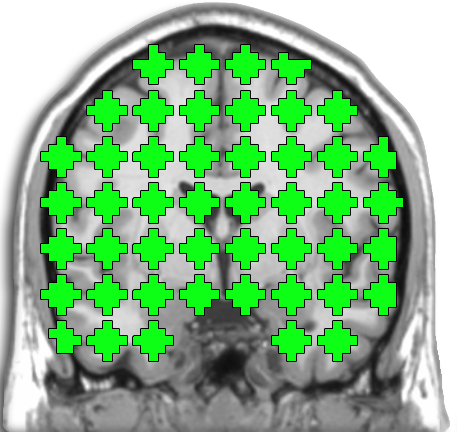
\includegraphics[height=100pt]{roi_slice_cor.png}
		\caption{Coronal}
	\end{subfigure}\hspace{12pt}
	\begin{subfigure}[t]{\imwidth}
		\centering
		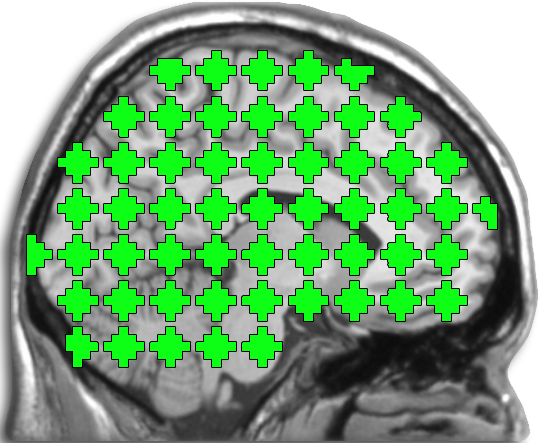
\includegraphics[height=100pt]{roi_slice_sag.png}
		\caption{Sagittal}
	\end{subfigure}\hspace{12pt}
	\begin{subfigure}[t]{\imwidth}
		\centering
		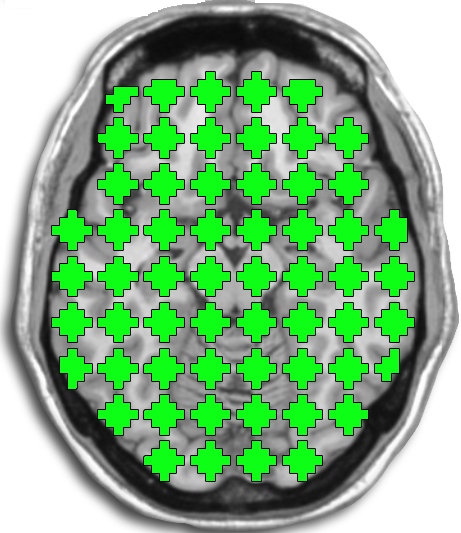
\includegraphics[height=100pt]{roi_slice_axi.png}
		\caption{Axial}
	\end{subfigure}
	\begin{subfigure}[t]{\imwidthh}
		\centering
		\raisebox{15pt}{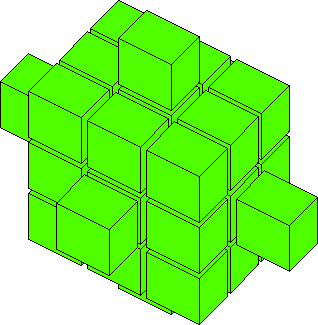
\includegraphics[height=60pt]{roi_pic}}
		\caption{Node (33 voxels)}
	\end{subfigure}
	\caption{
	Coronal, sagittal, and axial slices depicting the coverage of our brain parcellation scheme along with $3$-D rendering of one pseudo-sphereical node. 
	Each contiguous green region represents a pseudo-spherical node representing an ROI containing $33$-voxels.
	Overall, there are $347$ non-overlapping nodes placed throughout the entire brain.
	These nodes are placed on a grid with $18$ mm spacing between node centers in the $X$, $Y$, and $Z$ dimensions.
	}
	\label{fig:roi,grid,slice}
\end{figure}


%===================================================================%
% Statistical learning in high dimension
% * Supervised learning problem and margin based loss
% * Penalized empirical risk minimization and feature selection
% * Feature selection with spatial information
%===================================================================%
%!TEX root = paper.tex
\subsection{Statistical learning framework}
We now formally introduce the statistical learning framework adopted to perform joint feature selection and disease prediction with spatial information taken into consideration.

\subsubsection{Regularized empirical risk minimization and feature selection}
In this work, we are interested in the supervised learning problem of linear binary classification.
Suppose we are given a set of training data \sloppy{$\left\{(\x_1,y_1),\cdots,(\x_n,y_n)\right\}$}, where $\x_i\in\reals^p$ is the input feature vector and ${y_i\in\{-1,+1\}}$ is the corresponding class label for each $i\in[n]$.
In our application, $\x_i$ represents functional connectome and $y_i$ indicates the diagnostic status of subject $i\in[n]$, where we adopt the convention of letting $y=+1$ indicate ``disorder'' and $y=-1$ indicate ``healthy'' in this article.
The goal is to learn a linear decision function $\sign{\inprod{\x,\w}}$, parameterized by weight vector $\w\in\reals^p$, that predicts the label $y\in\{-1,+1\}$ of a new input $\x\in\reals^p$.
A standard approach for estimating \w is solving a regularized empirical risk minimization (ERM) problem with the form 
\begin{equation}
	\argmin{\w\in\reals^p} \frac{1}{n} \sum_{i=1}^n \loss\left(y_i \inprod{\w,\x_i}\right) + \lambda\Reg(\w) \;.
	\label{eqn:reg,erm}
\end{equation}
The first term $\frac{1}{n}\sum_{i=1}^n \loss\left(y_i \inprod{\w,\x_i}\right)$ corresponds to the \emph{empirical risk} of a margin-based loss function $\loss:\reals\to\reals_+$ (\eg, hinge, logistic, exponential), which quantifies how well the model fits the data.
The second term $\Reg:\reals^p\to\reals_+$ is a \emph{regularizer} that curtails overfitting and enforces some kind of structure on the solution by penalizing weight vectors that deviate from the assumed structure.
The user-defined regularization parameter $\lambda\geq0$ controls the tradeoff between data fit and regularization. 
Throughout this work, we assume the loss function and the regularizer to be convex, but not necessarily differentiable.
Furthermore, we introduce the following notations 
\[
	\begin{array}{ccc}
		\Y:=\diag{y_1,\cdots,y_n}			, &
		\X:=\ba{c} \x_1^T \\ \vdots \\ \x_n^T \ea , &
		\YXw=\ba{c} y_1 \inprod{\w,\x_1} \\ \vdots \\ y_n \inprod{\w,\x_n} \ea ,
	\end{array}
\]
which allow us to express the empirical risk succinctly by defining a functional \sloppy{${\Loss:\reals^n\to\reals_+}\;$} which aggregates the total loss ${\Loss(\YXw):=\sum_{i=1}^n \loss(y_i \inprod{\w,\x_i})}\,$.

Regularized ERM \eqref{eqn:reg,erm} has a rich history in statistics and machine learning, and many well known estimators can be recovered from this framework.
For example, when the hinge loss ${\loss(t):=\text{max}(0,1-t)}$ is used with the smoothness promoting \elltwo-regularizer $\norm{\w}^2_2$, we recover the SVM \citep{Cortes:1995}.
However, while smoothness helps prevent overfitting, it is problematic for model interpretation, as all the coefficients from the weight vector contribute to the final prediction function.
Automatic feature selection can be done using the \ellone-regularizer $\norm{\w}_1$ known as the Lasso \citep{Tibshirani:1996}, which causes many of the coefficients in \w to be exactly zero.
Because the prediction function is described by a linear combination between the weight \w and the feature vector \x, we can directly identify and visualize the regions that are relevant for prediction.

While the \ellone-regularizer possesses many useful statistical properties, several works have reported poor performance when the features are highly correlated.
More precisely, if there are clusters of correlated features, Lasso will select only a single representative feature from each cluster group, ignoring all the other equally predictive features.
This leads to a model that is overly sparse and sensitive to data resampling, creating problems for interpretation.
To address this issue, \cite{Zou:2005} proposed to combine the \ellone and \elltwo regularizers, leading to the Elastic-net, which has the form $\norm{\w}_1+\frac{\gamma}{2\lambda}\norm{\w}^2_2$, where $\gamma\geq 0$ is a second regularization parameter. 
The \ellone-regularizer has the role of encouraging sparsity, whereas the \elltwo-regularizer has the effect of allowing groups of highly correlated features to enter the model together, leading to a more stable and arguably a more sensible solution.  
While Elastic-net addresses part of the limitations of Lasso and has been demonstrated to improve prediction accuracy \citep{Carroll:2009,Ryali:2010}, it does not leverage the $6$-D structure of connectome space.  To address this issue, we employ the fused Lasso and GraphNet \citep{Grosenick:2013}.

%===================================================================%
% Structured sparsity with spatial information
%===================================================================%
\subsubsection{Spatially informed feature selection and classification via fused Lasso and GraphNet}
The original formulation of fused Lasso \citep{Tibshirani:2005} was designed for encoding correlations among successive variables in $1$-D data, such as mass spectrometry and comparative genomic hybridization (CGH) data \citep{Gui-Bo-Ye:2011}.
More specifically, assuming the weight vector $\w\in\reals^p$ has a natural ordering among its coordinates $j\in[p]$, the regularized ERM problem with the fused Lasso has the following form:
\begin{equation}
	\argmin{\w\in\reals^p}\frac{1}{n}\Loss(\YXw) + \lambda\norm{\Bw}_1 + 
		\gamma\sum_{j=2}^p\abs{w^{(j)} - w^{(j-1)}} \;,
	\label{eqn:fused,lasso,1d}
\end{equation}
where $w^{(j)}$ indicates the $j$-th entry of \w.
Like Elastic-net, this regularizer has two components: the first component is the usual sparsity promoting \ellone-regularizer, and the second component penalizes the absolute deviation among adjacent coordinates.
Together, they have the net effect of promoting sparse and piecewise constant solutions.

The idea of penalizing the deviations among neighboring coefficients can be extended to other situations where there is a natural ordering among the feature coordinates.
For instance, the extension of the $1$-D fused Lasso \eqref{eqn:fused,lasso,1d} for $2$-D imaging data is to penalize the \emph{vertical} and \emph{horizontal} difference between pixels; here, the coordinates are described via lexicographical ordering.
This type of generalization applies to our \mbox{$6$-D} functional connectomes by the virtue of the grid pattern in the nodes, and the ERM formulation reads
\begin{equation}
	\argmin{\w\in\reals^p}\frac{1}{n}\Loss(\YXw) + \lambda\norm{\Bw}_1 + 
		\gamma\sum_{j=1}^p\sum_{k\in\mathcal{N}_j} \abs{\;w^{(j)}-w^{(k)}} \;,
	\label{eqn:fused,lasso,6d}
\end{equation}
where $\mathcal{N}_j$ is the first-order neighborhood set corresponding to coordinate $j$ in \mbox{$6$-D} connectome space.
The spatial penalty $\gamma\sum_{j=1}^p\sum_{k\in\mathcal{N}_j} \abs{\,w^{(j)}-w^{(k)}}$ accounts for the \mbox{$6$-D} structure in the connectome by penalizing deviations among \emph{nearest-neighbor} edges, encouraging solutions that are spatially coherent in the connectome space.
This type of regularizer is known as an anisotropic total variation (TV) penalty in the image processing community \citep{Wang:2008tv}, and an analogous isotropic TV penalty was applied by \cite{Michel:2011} for the application of $3$-D brain decoding.

When the absolute value penalty in the spatial regularizer ${|\,w^{(j)}-w^{(k)}|}$ in \eqref{eqn:fused,lasso,6d} is replaced by the squared penalty $\frac{1}{2}(w^{(j)}-w^{(k)})^2$, we recover the GraphNet model proposed by \mbox{\cite{Grosenick:2013}}:
\begin{equation}
	\argmin{\w\in\reals^p}\frac{1}{n}\Loss(\YXw) + \lambda\norm{\Bw}_1 + 
		\frac{\gamma}{2}\sum_{j=1}^p\sum_{k\in\mathcal{N}_j} \left(w^{(j)}-w^{(k)}\right)^2 \;.
	\label{eqn:graphnet}
\end{equation}
GraphNet also promotes spatial contiguity, but instead of promoting sharp piecewise constant patches, it encourages the clusters to appear in smoother form by penalizing the quadratic deviations among the nearest-neighbor edges (\ie, the coordinates of the functional connectome \x).
We emphasize that the optimization algorithm we propose can be used to solve both fused Lasso~\eqref{eqn:fused,lasso,6d} and GraphNet~\eqref{eqn:graphnet} with very little modification.

To gain a better understanding of the neighborhood set $\mathcal{N}_j$ in the context of our application, let us denote $(x,y,z)$ and $(x',y',z')$ the pair of $3$-D points in the brain that define the connectome coordinate $j$.
Then, the first-order neighborhood set of $j$ can be written precisely as
\footnote{If $(x,y,z)$ or $(x',y',z')$ are on the boundary of the brain volume, then neighboring points outside the brain volume are excluded from $\mathcal{N}_j$.}
\begin{equation}
	\mathcal{N}_j:=
	\braces{
	\begin{array}{l}
			\big(x\pm 1,y,z,x',y',z'\big), \;
			\big(x,y\pm 1,z,x',y',z'\big), \;
			\big(x,y,z\pm 1,x',y',z'\big),\\
			\big(x,y,z,x'\pm 1,y',z'\big), \;
			\big(x,y,z,x',y'\pm 1,z'\big), \;
			\big(x,y,z,x',y',z'\pm 1\big)
	\end{array}}\; .
	\nonumber
\end{equation}
Fig.~\ref{fig,conn,neighbor} provides a pictorial illustration of $\mathcal{N}_j$ in the case of a $4$-D connectome, where the nodes reside in $2$-D space.

There are multiple reasons why fused Lasso and GraphNet are justified approaches for our problem.
For example, fMRI is known to possess high spatio-temporal correlation between neighboring voxels and time points, partly for biological reasons as well as from preprocessing (\eg, spatial smoothing).
Consequently, functional connectomes contain rich correlations among nearby coordinates in the connectome space.
In addition, there is a neurophysiological basis for why the predictive features are expected to be spatially contiguous rather than being randomly dispersed throughout the brain; this point will be  thoroughly discussed in Sec.~\ref{subsec:why,flasso}.
Finally, the spatial coherence that fused Lasso and GraphNet promote helps decrease model complexity and facilitates interpretation.

Letting $\C\in\reals^{e\times p}$ denote the $6$-D \emph{finite differencing matrix} (also known as the \emph{incidence matrix}), the spatial regularization term for both fused Lasso and GraphNet can be written compactly as
\begin{equation}
	\norm{\C\w}_q^q=\sum_{j=1}^p\sum_{k\in\mathcal{N}_j} |\,w^{(j)}-w^{(k)}|^q,\;\;\; q\in\{1,2\} \;,
	\nonumber
\end{equation}
where each row in \C contains a single $+1$ and a $-1$ entry, and $e$ represents the total number of adjacent coordinates in the connectome.
This allows us to write out the regularized ERM formulation for both fused Lasso~\eqref{eqn:fused,lasso,6d} and GraphNet~\eqref{eqn:graphnet} in the following unified form: 
\begin{equation}
	\argmin{\w\in\reals^p} \frac{1}{n}\Loss(\YXw) + \lambda\norm{\w}_1 + \frac{\gamma}{q}\norm{\C\w}^q_q  \; ,\; q\in\{1,2\}\;.
	\label{eqn:costfx}
\end{equation}
We will focus on this matrix-vector representation hereafter, as it is more intuitive and convenient for analyzing the variable splitting framework in the upcoming section.

%************************ Tikz fig ******************************%
\begin{figure}
	{\begin{center}
	\resizebox{0.39\linewidth}{!}{%!TEX root = paper.tex
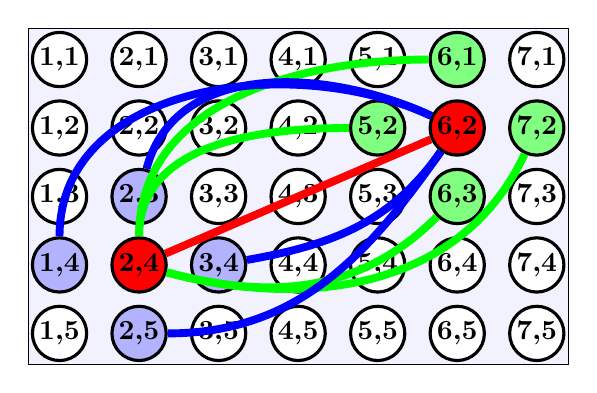
\begin{tikzpicture}[-,red, line width=0.1cm,font=\bfseries,draw=black] 
	\tikzstyle{every node}=[circle,ultra thick,draw=black,fill=white,text=black,minimum size=0cm,line width=0.04cm,inner sep=1pt]
	\tikzstyle{main} =[fill=red]
	\tikzstyle{main1} =[fill=blue!30]
	\tikzstyle{main2} =[fill=green!50]
	\matrix [rectangle,row sep=4pt, column sep=8pt,draw=black,fill=blue!5,line width=0.01cm] % 
	{
	\node  (1_1){1,1} ;& 	\node  (1_2) {2,1} ;&	\node  (1_3) {3,1} ;&	\node  (1_4) {4,1} ;&	\node  (1_5) {5,1} ;&	\node  (MAIN2T)[main2] {6,1}  ;&	\node  (1_7) {7,1} ;\\
	\node  (2_1){1,2} ;& 	\node  (2_2) {2,2} ;&	\node  (2_3) {3,2} ;&	\node  (2_4) {4,2} ;&	\node  (MAIN2L)[main2] {5,2} ;&	\node  (MAIN2)[main] {6,2} ;&	\node  (MAIN2R)[main2] {7,2} ;\\
	\node  (3_1){1,3} ;& 	\node  (MAIN1T)[main1] {2,3} ;&	\node  (3_3) {3,3} ;&	\node  (3_4) {4,3} ;&	\node  (3_5) {5,3} ;&	\node  (MAIN2B)[main2] {6,3} ;&	\node  (3_7) {7,3} ;\\
	\node(MAIN1L)[main1]  {1,4} ;& 	\node  (MAIN1)[main]{2,4} ;&	\node  (MAIN1R)[main1] {3,4} ;&	\node  (4_4) {4,4} ;&	\node  (4_5) {5,4} ;&	\node  (4_6) {6,4} ;&	\node  (4_7) {7,4} ;\\
	\node  (5_1){1,5} ;& 	\node  (MAIN1B)[main1] {2,5} ;&	\node  (5_3) {3,5} ;&	\node  (5_4) {4,5} ;&	\node  (5_5) {5,5} ;&	\node  (5_6) {6,5} ;&	\node  (5_7) {7,5} ;\\
};
	\draw (MAIN1) to (MAIN2) [red];

	\draw[green] (MAIN1) to [out=90,in=180] (MAIN2L) ;
	\draw[green] (MAIN1) to [out=90,in=180] (MAIN2T) ;
	\draw[green] (MAIN1) to [out=-15,in=-115] (MAIN2R) ;
	\draw[green] (MAIN1) to [out=-15,in=-135](MAIN2B) ;
	
	\draw[blue] (MAIN2) to  [out=155,in=90] (MAIN1L) ;
	\draw[blue] (MAIN2) to  [out=155,in=75](MAIN1T) ;
	\draw[blue] (MAIN2) to [out=-125,in=10](MAIN1R) ;
	\draw[blue] (MAIN2) to [out=-125,in=0](MAIN1B) ;
\end{tikzpicture}
}\\
	\textbf{{$\mathcal{N}_j$ in $\bmath{4}$-D Connectome Space}} \vspace{-15pt}\\
	\end{center}	
	}
	\caption{
	Illustration of the neighborhood structure of the connectome when the nodes reside in $2$-D space.  
	The red edge represents coordinate $j=\big\{(2,4),(6,2)\big\}$ in $4$-D connectome space, and its neighborhood set $\mathcal{N}_j$ is represented by the blue and green edges.  
	This idea extends directly to $6$-D connectomes generated from $3$-D resting state volumes.
	}
	\label{fig,conn,neighbor}
\end{figure}
%******************************************************************%


%===================================================================%
% Optimization method
% - primer on admm
% - variable splitting setup
% - closed form admm updates
%===================================================================%
\subsection{Optimization}\label{subsec:optim}
%!TEX root = paper.tex
%===================================================================%
% Optimization
%===================================================================%
Solving the optimization problem \eqref{eqn:costfx} is challenging since the problem size $p$ is large and the three terms {in the cost function} can each be \mbox{non-differentiable}.
To address these challenges, we now introduce a scalable optimization framework based on augmented Lagrangian (AL) methods.
In particular, we introduce a variable splitting scheme that converts the unconstrained optimization problem of the form \eqref{eqn:costfx} into an equivalent constrained optimization problem, which can be solved efficiently using the alternating direction method of multipliers (ADMM) algorithm \citep{Boyd:2011,Glowinski:1975, Gabay:1976}. 
We demonstrate that by augmenting the weight vector with zero entries at appropriate locations, the inner subproblems associated with ADMM can be solved efficiently in closed form.

%===================================================================%
\subsubsection{Alternating Direction Method of Multipliers}
The ADMM algorithm is a powerful algorithm for solving convex optimization problems having the separable structure \citep{Boyd:2011}
\begin{equation}
	\minimize{\xbar,\ybar}\,\fbar(\xbar) + \gbar(\ybar) \;\;\;\; 
	\text{subject to } \Abar\xbar+\Bbar\ybar=\bzero \;,
	\label{eqn:canonical,admm}
\end{equation}
where $\xbar\in\reals^\pbar$ and $\ybar\in\reals^\qbar$ are unknown primal variables, $\fbar:\reals^\pbar\to\reals\cup\{+\infty\}$ and $\gbar:\reals^\qbar\to\reals\cup\{+\infty\}$ are closed convex functions, and $\Abar\in\reals^{c\times \pbar}$ and $\Bbar\in\reals^{c\times \qbar}$ are matrices representing $c$ linear constraints.  
More specifically, the ADMM algorithm solves for the primal variables in \eqref{eqn:canonical,admm} through the following iterative procedure:
\begin{align}
	&\hspace{0.17\linewidth}\xbar\iterp\leftarrow\displaystyle\argmin{\xbar} \fbar(\xbar) + \frac{\rho}{2}\norm{\Abar\xbar + \Bbar\ybar\iter + \u\iter}^2 \label{eqn:admm,xbar,update}\\ 
	&\hspace{0.17\linewidth}\ybar\iterp\leftarrow\displaystyle\argmin{\ybar} \gbar(\ybar) + \frac{\rho}{2}\norm{\Abar\xbar\iterp + \Bbar\ybar + \u\iter}^2 \label{eqn:admm,ybar,update}\\ 
	&\hspace{0.17\linewidth}\u\iterp\leftarrow \u\iter+ \left(\Abar\xbar\iterp+\Bbar\ybar\iterp\right)  \; , & \label{eqn:admm,dual,update}
\end{align}
where superscript $t$ denotes the iteration count and $\u\in\reals^c$ denotes the (scaled) dual variable.

The convergence of the ADMM algorithm has been established in Theorem $1$ of \cite{Mota:2011}, which states that if matrices \Abar and \Bbar are full column-rank and the problem \eqref{eqn:canonical,admm} is solvable (\ie, it has an optimal objective value), the ADMM iterations \eqref{eqn:admm,xbar,update} - \eqref{eqn:admm,dual,update} converges to the optimal solution.
While the AL parameter $\rho>0$ does not affect the convergence property of ADMM, it can impact its convergence speed.
We use the value $\rho=1$ in all of our implementations.

%===================================================================%
\subsubsection{Variable splitting and data augmentation}
\label{subsec:var,split}
The original formulation of our problem \eqref{eqn:costfx} does not have the structure of \eqref{eqn:canonical,admm}.
However, we can convert the unconstrained optimization problem \eqref{eqn:costfx} into an equivalent constrained optimization problem \eqref{eqn:canonical,admm} by introducing auxiliary constraint variables, a method known as \emph{variable splitting} \citep{Afonso:2010}.  
While there are several different ways to introduce the constraint variables, the heart of the strategy is to select a splitting scheme that decouples the problem into more manageable subproblems.
For example, one particular splitting strategy we can adopt for problem \eqref{eqn:costfx} is
\begin{equation}
	\begin{array}{c}
		\dstyle\minimize{\substack{\w,\va \\ \vb,\vc,\vd}} 
			\frac{1}{n}\Loss(\va)+\lambda\norm{\vb}_1+\frac{\gamma}{q}\norm{\vc}^q_q \; \; 
			\vspace{0.01\linewidth}\\
		\text{ subject to }  \YXw =\va, \; \w=\vb, \; \C\vd=\vc, \;  \w=\vd \;, 
	\end{array}
	\label{eqn:splitting1}
\end{equation}
where $\va,\vb,\vc,\vd$ are the constraint variables.
It is easy to see that problems \eqref{eqn:costfx} and \eqref{eqn:splitting1} are equivalent, and the correspondence with the ADMM formulation \eqref{eqn:canonical,admm} is as follows:
\begin{equation}
	\begin{array}{c}
		\fbar(\xbar)=\dstyle\frac{\gamma}{q}\norm{\vc}^q_q , \;\;\;
		\gbar(\ybar)=\dstyle\frac{1}{n}\Loss(\va) + \lambda\norm{\vb}_1  
		\vspace{0.02\linewidth} \\
		\Abar = 	\ba{cc} 	\Y\X	& \bzero \\ \I	& \bzero \\ \bzero 	& \I \\ \I & \bzero \ea 	, \;
		\xbar = \bmat \w \\ \vc \emat, 
		\Bbar = 	\ba{rrr} 	-\I 	& \bzero	& \bzero \\ \bzero & -\I & \bzero  \\ 
						 \bzero & \bzero & -\C \\ \bzero & \bzero & -\I \ea,
		\ybar = \bmat \va \\ \vb \\ \vd \emat 	.
	\end{array}
	\label{eqn:admm,objective1}
\end{equation}
However, there is an issue with this splitting strategy: one of the resulting subproblems from the ADMM algorithm requires us to invert a matrix involving the Laplacian matrix $\C^T\C\in\reals^{p\times p}$, which is prohibitively large.
Although this matrix is sparse, it has a distorted structure due to the irregularities in the coordinates of \x.
These irregularities arise from two reasons:
(1) the nodes defining the functional connectome \x are placed only on the brain, not the entire rectangular field of view (FOV), and
(2) \x lacks a complete $6$-D representation since it only contains the lower-triangular part of the cross-correlation matrix.
Fig.~\ref{fig:lap,noncirc} displays the Laplacian matrix that results from the $347$-node functional connectome defined in Section~\ref{subsec:FC,def}, and the distorted structure is clearly visible.

To address this issue, we introduce an \emph{augmentation matrix} $\A\in\reals^{\ptil\times p}$, whose rows are either the zero vector or an element from the trivial basis $\braces{\bmath{e}_j \; |\; j\in[p]}$, and has the property $\A^T\A=\I_p$.
Furthermore, we define the \emph{augmented weight vector} $\wtil:=\A\w$, where \A rectifies the irregularities in the coordinates of \w (and \x) by padding extra zero entries, accommodating for:
(1) the nodes that were not placed in the FOV (\ie, the regions outside the brain), and
(2) the diagonal and upper-triangular part of the cross-correlation matrix, which were disposed due to redundancy; further details regarding this augmentation scheme is reported in \ref{appendix:data,aug}.
As a result, we now have a new differencing matrix $\Ctil\in\reals^{\tilde{e}\times\ptil}$ corresponding to $\wtil\in\reals^\ptil$, whose Laplacian matrix $\Ctil^T\Ctil\in\reals^{\ptil\times\ptil}$ has a systematic structure, as shown in Fig.~\ref{fig:lap,circ}.
In fact, this matrix has a special structure known as \emph{block-circulant with circulant-blocks} (BCCB), which is critical since the matrix inversion involving $\Ctil^T\Ctil$ can be computed efficiently in closed form using the fast Fourier transform (FFT) (the utility of this property will be elaborated more in Section~\ref{subsec:admm,steps}).  
It is important to note that this BCCB structure in the Laplacian matrix arises from the grid structure introduced from the parcellation scheme we adopted for producing the functional connectome.

%********** Laplacian matrix figures ****************%
\renewcommand{\imwidth}  {0.38\linewidth}
\begin{figure}
	\centering
	\begin{subfigure}[t]{\imwidth}
		 \centering
		 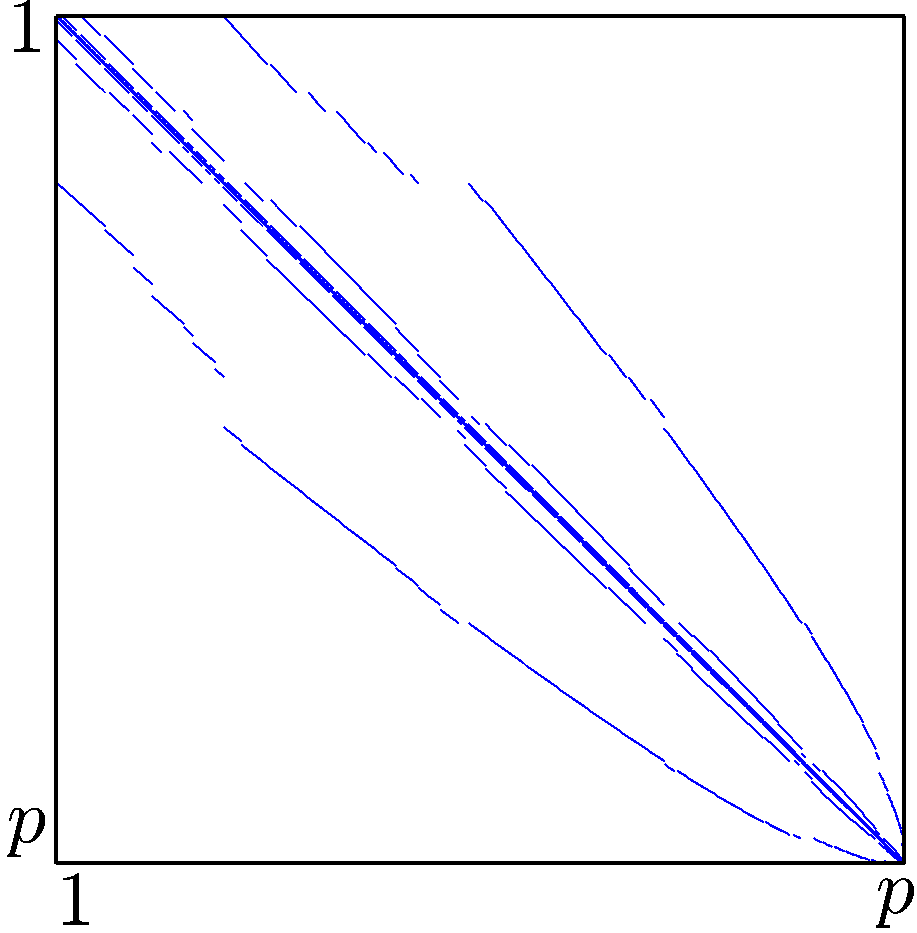
\includegraphics[height=.7\linewidth]{laplacemat_noncirc.pdf}
		 \caption{Laplacian matrix: $\C^T\C$}
		 \label{fig:lap,noncirc}
	\end{subfigure}
%	\hfill
	\hspace{0.05\linewidth}
	\begin{subfigure}[t]{\imwidth}
		 \centering
		 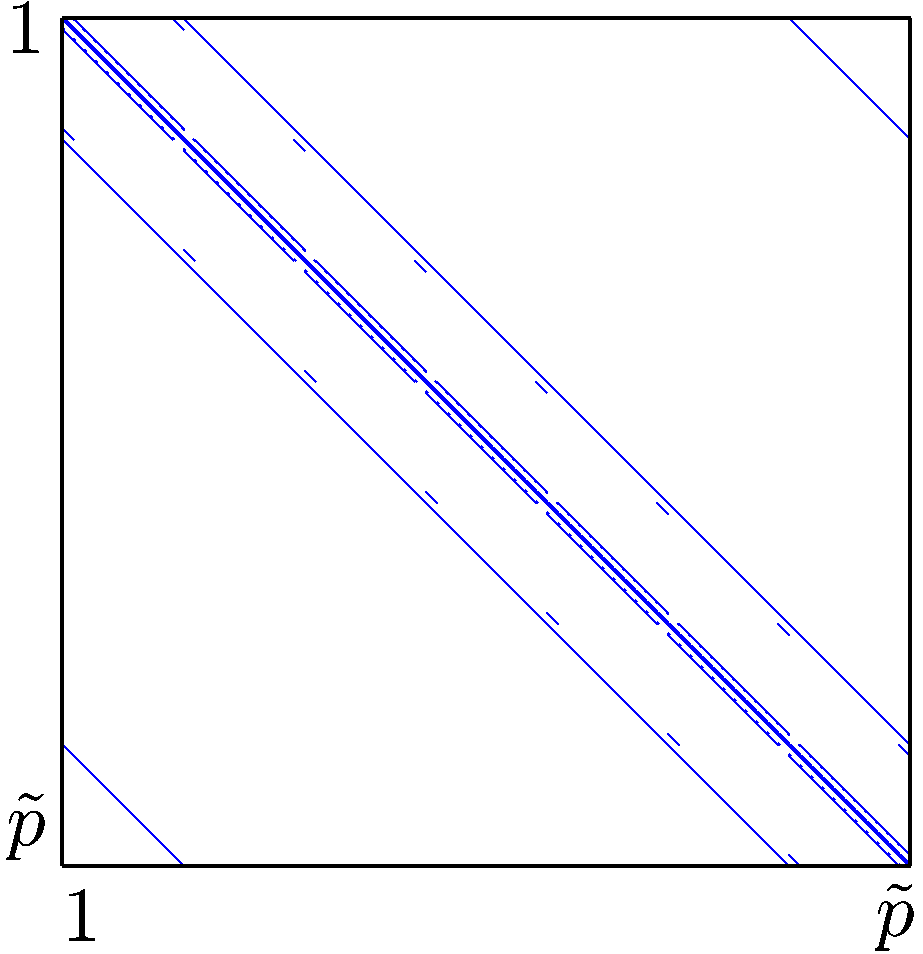
\includegraphics[height=.7\linewidth]{laplacemat_circ.pdf}
		 \caption{Augmented Laplacian matrix: $\Ctil^T\Ctil$}
		 \label{fig:lap,circ}
	\end{subfigure}

	\caption{Laplacian matrix corresponding to the original data $\C^T\C$ and the augmented data $\Ctil^T\Ctil$, where the rows and columns of these matrices represent the coordinates of the original and augmented functional connectome.  Note that the irregularities in the original Laplacian matrix are rectified by data augmentation.  The augmented Laplacian matrix has a special structure known as \emph{block-circulant with circulant-blocks} (BCCB), which has important computational advantages that will be exploited in this work.}
	 \label{fig:lap}
\end{figure}
%********************************************************%

Finally, by introducing a diagonal masking matrix $\B\in\{0,1\}^{\ptil\times\ptil}$, we have $\|\B\Ctil\wtil\|^q_q = \norm{\C\w}_q^q$ for $\q\in\{1,2\}$.  
Note that this masking strategy was adopted from the recent works of \cite{Allison:2013} and \cite{Matakos:2013}, and has the effect of removing artifacts that are introduced from the data augmentation procedure when computing the $\norm{\cdot}_q^q$-norm.
This allows us to write out the fused Lasso and GraphNet problem \eqref{eqn:costfx} in the following equivalent form:
\begin{equation}
	\argmin{\w\in\reals^p} \frac{1}{n}\Loss(\YXw) + \lambda\norm{\w}_1 + 
		\frac{\gamma}{q}\norm{\B\Ctil\A\w}^q_q  \; ,\; q\in\{1,2\}
	\nonumber
\end{equation}
Moreover, this can be converted into a constrained optimization problem
\begin{equation}
	\begin{array}{c}
		\dstyle\minimize{\substack{\w,\va \\ \vb,\vc,\vd}} 
			\frac{1}{n}\Loss(\va)+\lambda\norm{\vb}_1+\frac{\gamma}{q}\norm{\B\vc}^q_q \; \; 
			\vspace{0.01\linewidth}\\
		\text{ subject to }  \YXw =\va, \; \w=\vb, \; \Ctil\vd=\vc, \;  \A\w=\vd \;, 
	\end{array}
	\label{eqn:admm,splitting2}
\end{equation}
and the correspondence with the ADMM formulation \eqref{eqn:canonical,admm} now becomes:
\begin{equation}
	\begin{array}{c}
		\fbar(\xbar)=\dstyle\frac{\gamma}{q}\norm{\B\vc}^q_q , \;\;\;
		\gbar(\ybar)=\dstyle\frac{1}{n}\Loss(\va) + \lambda\norm{\vb}_1  
		\vspace{0.02\linewidth} \\
		\Abar = 	\ba{cc} 	\Y\X	& \bzero \\ \I	& \bzero \\ \bzero 	& \I \\ \A & \bzero \ea 	, \;
		\xbar = \bmat \w \\ \vc \emat 			, 
		\Bbar = 	\ba{rrr} 	-\I 	& \bzero	& \bzero \\ \bzero & -\I & \bzero  \\ 
						 \bzero & \bzero & -\Ctil \\ \bzero & \bzero & -\I \ea 		, 
		\ybar = \bmat \va \\ \vb \\ \vd \emat \;.
	\end{array}
	\label{eqn:admm,objective2}
\end{equation}
The dual variables corresponding to $\va,\vb,\vc,$ and $\vd$ are written in block form $\u=[\ua^T,\ub^T,\uc^T,\ud^T]^T$.
Note that functions \fbar and \gbar are convex, and matrices \Abar and \Bbar are full column-rank, so the convergence of the ADMM iterations \eqref{eqn:admm,xbar,update}-\eqref{eqn:admm,dual,update} is guaranteed (see Theorem~1 in \cite{Mota:2011}).

%===================================================================%
\subsubsection{ADMM: efficient closed-form updates}
\label{subsec:admm,steps}

With the variable splitting scheme \eqref{eqn:admm,splitting2} and ADMM formulation \eqref{eqn:admm,objective2}, the ADMM update for the primal variable $\xbar$ \eqref{eqn:admm,xbar,update} decomposes into subproblems
\begin{alignat}{1} 
	\w\iterp 	\leftarrow \argmin{\w}&
		 \Bigg\{\normsq{\Y\X\w-\left(\va\iter-\ua\iter\right)} 
		+ \normsq{\w-\left(\vb\iter-\ub\iter\right)} \nonumber \\
		  &+ \normsq{\A\w-\left(\vd\iter-\ud\iter\right)} \Bigg\} \label{eqn:w,update1} \\
	\vc\iterp \leftarrow \argmin{\vc}&
		\Bigg\{\frac{\gamma}{q}\norm{\B\vc}_q^q
		  +\frac{\rho}{2}\normsq{\vc-\left(\Ctil\vd\iter-\uc\iter\right)}\Bigg\}\;, \label{eqn:v3,update1}
\end{alignat}
whereas the updates for primal variable $\ybar$ \eqref{eqn:admm,ybar,update} are
\begin{alignat}{1} 
	\va\iterp \leftarrow \argmin{\va}
		& \left\{ \frac{1}{n}\Loss(\va) + \frac{\rho}{2}\normsq{\va-\left(\Y\X\w\iterp+\ua\iter\right)} \right\}
			\label{eqn:v1,update1}\\
	\vb\iterp \leftarrow \argmin{\vb} 
		& \left\{\lambda\norm{\vb}_1 + \frac{\rho}{2}\normsq{   \vb-\left(\w\iterp+\ub\iter\right)} 
			\label{eqn:v2,update1}\right\}\\
	\vd\iterp \leftarrow \argmin{\vd}
		& \bigg\{\normsq{\Ctil\vd-\left(\vc\iterp+\uc\iter\right)}
		 + \normsq{\vd-\left(\A\w\iterp+\ud\iter\right)}\bigg\} \;.  \label{eqn:v4,update1}
\end{alignat}
The update for the dual variable \u is a trivial matrix-vector \mbox{multiplication \eqref{eqn:admm,dual,update}} (see Algorithm~\ref{alg:admm} line $14$-$17$).

We now demonstrate that the minimization problems \eqref{eqn:w,update1}-\eqref{eqn:v4,update1} each admits an efficient, closed form solution.

\newcommand{\Bvarrho}{\bmath{\varrho}}
%--------------------------------------------------%
\paragraph{\w update}
The quadratic minimization problem \eqref{eqn:w,update1} has the following closed form solution:
\begin{align}
	\w\iterp \leftarrow \left(\X^T\X + 2\BI_p\right)\inv  
		\Big(&\X^T\Y^T [\va\iter-\ua\iter] 
		+[\vb\iter-\ub\iter]  
		 +\A^T[\vd\iter-\ud\iter] \Big) \,. \label{eqn:w,update2}
\end{align}
Note we used the fact that $\Y^T\Y=\I_n$ and $\A^T\A=\I_p$ to arrive at this expression.
Applying update \eqref{eqn:w,update2} brute force will require an inversion of a $(p\times p)$ matrix, but this can be converted into an $(n\times n)$ inversion problem by invoking the \emph{matrix inversion Lemma}
\begin{equation}
	\left( \X^T\X + 2\BI_p   \right)\inv = 
	\frac{1}{2}\I_p - \frac{1}{4}\X^T \big( \I_n + \frac{1}{2}\X\X^T \big)\inv\X \; .
	\label{eqn:inv,lemma}
\end{equation}
In the context of our work, $n$ denotes the number of scanned subjects, which is typically on the order of a few hundred.
The matrix $(\X^T\X + 2\BI_p)\inv$ can be stored in memory if $p$ is small, but the massive dimensionality of the functional connectome in our application dismisses this option.
Therefore, we instead precompute the $(p\times n)$ matrix $\BH:=\frac{1}{4}\X^T(\I_n+\frac{1}{2}\X\X^T)\inv$ in~\eqref{eqn:inv,lemma}, and let
\[\Bvarrho\iter:=\X^T\Y^T [\va\iter-\ua\iter] +[\vb\iter-\ub\iter] +\A^T[\vd\iter-\ud\iter]\;.\]
This way, the update \eqref{eqn:w,update2} can be implemented as follows:
\begin{equation}
	w\iterp \leftarrow(\X^T\X + 2\I_p)\inv\Bvarrho\iter=\frac{1}{2}\Bvarrho\iter - \BH\X\Bvarrho\iter\;,
	\label{eqn:inv,lemma2}
\end{equation}
which allows us to carry out the \w-update without having to store a $(p\times p)$ matrix in memory.

%--------------------------------------------------%
\paragraph{\va and \vb update}
The minimization problems \eqref{eqn:v1,update1} and \eqref{eqn:v2,update1} have the form of the (scaled) proximal operator $\prox_{\tau F}:\reals^p\to\reals^p$ \citep{Rockafellar:1998:book}, defined by 
\begin{equation}
	\prox_{\tau F}(\Bv)= \argmin{\Bu\in\reals^p}\tau F(\Bu)+\frac{1}{2}\norm{\Bv-\Bu}^2 ,\;\; \tau>0\;,
	\label{eqn:prox}
\end{equation}
where $F:\reals^p\to\reals\cup\{+\infty\}$ is a closed convex function.
Using standard subdifferential calculus rules \citep{Borwein:2006:book}, it is straightforward to show that a point $\u^*\in\reals^p$ solves the minimization in \eqref{eqn:prox} if and only if the condition 
\begin{equation}
	\bzero\in \partial F(\u^*)+(\u^*-\Bv)/\tau
	\label{eqn:prox,opt,cond}
\end{equation} 
holds.
Here, $\partial F(\u^*)$ denotes the subdifferential of function $F$ at $\u^*$, defined by 
\begin{equation}
	\partial F(\u^*):= \left\{ \Bz\in\reals^p :
		 F(\u^*) + \inprod{\Bz,\u-\u^*} \leq F(\u),\; \forall \u\in\reals^p
						\right\}     .
\nonumber
\end{equation}

In addition, both updates \eqref{eqn:v1,update1} and \eqref{eqn:v2,update1} are fully separable across their coordinates, decomposing into the following sets of elementwise scalar optimization problems:
\begin{alignat}{3} 
  \left[\va\iterp\right]_i \;\;\leftarrow \;\;&
  	\prox_{\frac{\loss}{n\rho}}\left(\big[ \Y\X\w\iterp + \ua\iter \big]_i\right) ,
  	& \;\;\;\;\;\; i\in[n] \label{eqn:v1,update2} \\
  \left[\vb\iterp\right]_j \;\;\leftarrow \;\;&
  	\prox_{\frac{\lambda}{\rho}\abs{\cdot}}\left(\big[ \w\iterp+\ub\iter \big]_j\right) ,
  	& j\in[p] &\;,\label{eqn:v2,update2} 
\end{alignat}
where $[\,\cdot\,]_i$ and $[\,\cdot\,]_j$ each index the $i$-th and $j$-th element of a vector in $\reals^n$ and $\reals^p$ respectively.
For some margin-based loss functions, their corresponding proximal operator \eqref{eqn:v1,update2} can be derived in closed form using the optimality condition~\eqref{eqn:prox,opt,cond}.
Fig.~\ref{fig:prox} plots a few commonly used margin-based losses and their corresponding proximal operators, and Table~\ref{table:prox} provides their closed form expressions.
The choice of the margin-based loss is application dependent, such as whether differentiability is desired or not.
The proximal operator of the \ellone-norm~\eqref{eqn:v2,update1} and the absolute loss function~\eqref{eqn:v2,update2} corresponds to the well known \emph{soft-threshold operator} \citep{Donoho:1995}
\begin{equation}
	\text{Soft}_\tau(t):=
		\begin{cases}
			t-\tau & \text{if } t > \tau \\
			0		& \text{if } \abs{t}\leq \tau \\
			t+\tau	& \text{if } t < -\tau
		\end{cases} \;\;.
	\label{eqn:soft,thresh}
\end{equation}
The absolute loss and the soft-threshold operator are also included in Fig.~\ref{fig:prox} and Table.~\ref{table:prox} for completeness.

% figure table of loss functions and prox functions in this work
%======================= Proximal operators =============================%
\afterpage{%    % defer execution until the next page break occurs anyway
\renewcommand{\imwidth}  {0.365\linewidth}
\renewcommand{\imwidthh}  {0.88\linewidth}
\begin{figure}[t!]
	\centering
	\begin{subfigure}[t]{\imwidth}
		 \centering
		 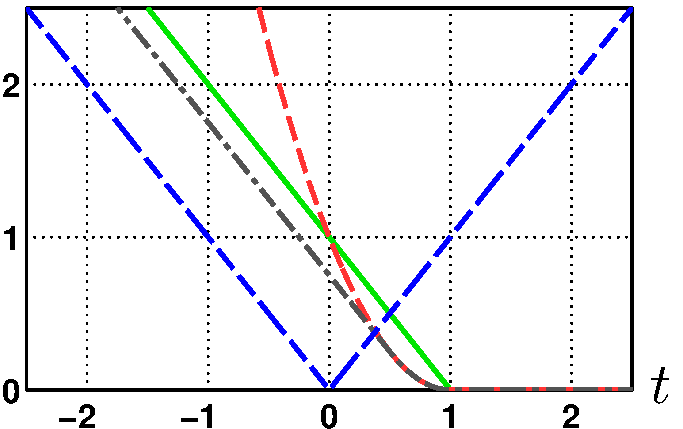
\includegraphics[width=\imwidthh]{prox_map_loss.pdf}
		 \caption{{Loss functions $\loss(t)$}}
		 \label{subfig:loss,fcn}
	\end{subfigure}
%	\hfill
	\begin{subfigure}[t]{0.225\linewidth}
		 \centering
		 \raisebox{0.17\linewidth}{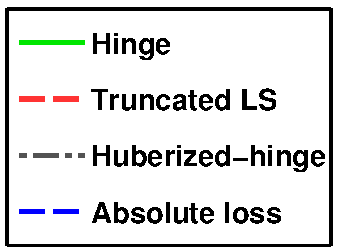
\includegraphics[width=\imwidthh]{prox_map_legend.pdf}}
	\end{subfigure}
%	\hfill
	\begin{subfigure}[t]{\imwidth}
		 \centering
		 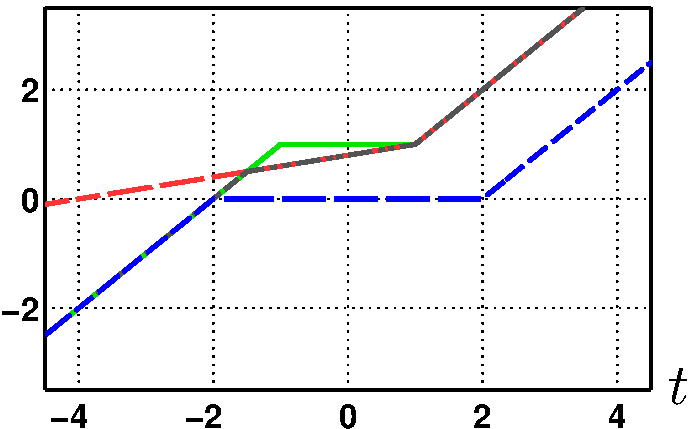
\includegraphics[width=\imwidthh]{prox_map_prox.pdf}
		 \caption{{Proximal operator $\prox_{\tau\loss}(t)$}}
		 \label{subfig:loss,prox}
	\end{subfigure}%
	\caption{Plots of scalar convex loss functions that are relevant in this work, along with their associated proximal operators. 
	  Table~\ref{table:prox} provides the closed form expression for these functions.  
	  Parameter values of $\tau=2$ and $\delta=0.5$ are used in the plot for the proximal operator and the huberized hinge-loss respectively.}
	\label{fig:prox}
\end{figure}
\begin{table}[h!]\small
	\centering
	\begin{tabular}{c|c|l}
		& \normalsize{$\loss(t)$} & \hspace{0.1\linewidth}\normalsize{$\prox_{\tau\loss}(t)$}\\
		\hline\hline  %<- requires the "booktabs" package
		 Hinge 			& $\max(0,1-t)$ 	& 
			 $\begin{cases}
				t 		& \text{if } t>1\\
				1 		& \text{if } 1-\tau\leq t \leq 1 \\
				t+\tau	& \text{if } t < 1-\tau
			 \end{cases}$\\ \hline
		 \begin{tabular}{c}Truncated\\ least squares\end{tabular}	
		 	& $\big\{\max(0,1-t)\big\}^2$	& 
		 	$\begin{cases}
		 		t			& \text{if } t>1 \\
		 		\dstyle\frac{t+2\tau}{1+2\tau}	& \text{if } t\leq 1 \\
		 	\end{cases}$\\ \hline
		  \begin{tabular}{c}Huberized\\ hinge \\ \citep{Wang:2008} \end{tabular}		& 
			 $\begin{cases}
				0 					&\text{if } t>1 \\
			 	\dstyle\frac{(1-t)^2}{2\delta} 	&\text{if } 1-\delta \leq t \leq 1 \\
			 	 1-t-\frac{\delta}{2}	&\text{if } t < 1-\delta
			 \end{cases}$
			 & 
			 $\begin{cases}
				t 		&\text{if } t>1 \\
			 	\dstyle\frac{t+\tau/\delta}{1+\tau/\delta} 	&\text{if } 1-\delta-\tau \leq t \leq 1 \\
			 	t+\tau	&\text{if } t < 1-\delta-\tau
			 \end{cases}$ \\ \hline
		 \begin{tabular}{c}Absolute \\ loss\end{tabular}	
		 	& \begin{tabular}{c}
		 		$\abs{t}$\\ (from \ellone-regularization)
		 	  \end{tabular}	
		 	  & 
			 $\text{Soft}_\tau(t):=
			 \begin{cases}
			 	t-\tau & \text{if } t > \tau \\
			 	0		& \text{if } \abs{t}\leq \tau \\
			 	t+\tau	& \text{if } t < -\tau
			 \end{cases}$ \\
		\hline
	\end{tabular}
	\caption{Examples of scalar convex loss functions that are relevant for this work, along with their corresponding proximal operators in closed form.}
	\label{table:prox}
\end{table}
} % end of argument of `\afterpage` command
%=========================================================================%

%--------------------------------------------------%
\paragraph{\vc update}
The solution to the minimization problem \eqref{eqn:v3,update1} depends on the choice of $q\in\{1,2\}$, where $q=1$ recovers fused Lasso and $q=2$ recovers GraphNet.

In the fused Lasso case $q=1$, since the masking matrix $\B\in\{0,1\}^{\ptil\times\ptil}$ is diagonal, the update~\eqref{eqn:v3,update1} is fully separable.
Letting $\Bzeta\iter:=\Ctil\vd\iter-\uc\iter$, the minimization problem decouples into a set of scalar minimization problems of the form:
\begin{equation}
	\argmin{v_k\in\reals}\left\{ \gamma\; b_k\abs{v_k} + 
			\frac{\rho}{2} \left(v_k-\zeta_k\iter \right)^2  
		\right\} \;,\;\;\;\; k\in[\ptil]
	\label{eqn:v3,scalar}
\end{equation}
where $b_k$ is the $k$-th diagonal entry of \B and $\zeta_k\iter$ is the $k$-th entry of \sloppy{${\Bzeta\iter\in\reals^\ptil}$}.
On one hand, when $b_k=0$, the minimizer for problem~\eqref{eqn:v3,scalar} returns the trivial solution $\zeta_k\iter$.
On the other hand, when $b_k=1$, the minimizer will once again have the form of the proximal operator~\eqref{eqn:prox} corresponding to the absolute loss function $\abs{\cdot}$, recovering the soft-threshold operator~\eqref{eqn:soft,thresh}.
To summarize, when $q=1$, the update for \vc \eqref{eqn:v3,update1} can be done efficiently by conducting the following elementwise update for each $k\in[\ptil]$:
\begin{equation}
	\left[\vc\iterp\right]_k \;\leftarrow
	\begin{cases}
		\soft_{\gamma/\rho}\left(\left[\Ctil\left(\vd\iter-\uc\iter\right)\right]_k\right) & \text{if } \B_{k,k}=1 \\
		\left[\Ctil\left(\vd\iter-\uc\iter\right)\right]_k & \text{if } \B_{k,k}=0
	\end{cases}	
	\label{eqn:v3,update,flasso}
\end{equation}
where $\left[\cdot\right]_k$ indexes the $k$-th element of a vector in $\reals^\ptil$.

In the GraphNet case $q=2$, update \eqref{eqn:v3,update1} is a quadratic optimization problem with the closed form solution
\begin{equation}
	\vc\iterp \leftarrow \rho\big(\gamma\B+\rho\I_\ptil)\inv\Ctil(\vd\iter-\uc\iter) \;,
	\label{eqn:v3,update,gnet}
\end{equation}
which is trivial to compute since the matrix $(\gamma\B+\rho\I_\ptil)$ is diagonal.

%===================================================================%
\paragraph{\vd update}

The closed form solution to the quadratic optimization problem \eqref{eqn:v4,update1} is 
\begin{equation}
	\vd\iterp \leftarrow \left(\Ctil^T\Ctil + \I_\ptil\right)\inv
		\left(\Ctil^T[\vc\iter+\uc\iter]+\A\w\iterp+\ud\iter\right) \;.
	\label{eqn:v4,update2}
\end{equation}
To suppress notations, let us define $\Q\in\reals^{\ptil\times\ptil}$ and $\b\in\reals^\ptil$, where
$\Q:=\Ctil^T\Ctil + \I_\ptil$
and 
\[\b:=\Ctil^T[\vc\iter+\uc\iter]+\A\w\iterp+\ud\iter .\]
As stated earlier, the Laplacian matrix $\Ctil^T\Ctil$ is block-circulant with circulant-blocks (BCCB), and consequently, the matrix \Q is BCCB as well.  
It is well known that a BCCB matrix can be diagonalized as \citep{Davis:1979:book}
	\[\Q=\U^H\BLambda\U,\]
where $\U\in\reals^{\ptil\times\ptil}$ is the ($6$-D) DFT matrix and $\BLambda\in\reals^{\ptil\times\ptil}$ is a diagonal matrix containing the ($6$-D) DFT coefficients of the first column of \Q .
As a result, the update \eqref{eqn:v4,update2} can be carried out efficiently using the (6-D) FFT 
\begin{equation}
 	\Q\inv\b = 
 		\left(\U^H \BLambda\inv \U\right)\b = 
 		\mathrm{ifft}\Big(	\mathrm{fft}(\b)\odiv\Bphi \Big) \;,
 	\label{eqn:v4,fft}
\end{equation}
where $\text{fft}$ and $\text{ifft}$ denote the ($6$-D) FFT and inverse-FFT operation\footnote{These multidimensional FFT and inverse FFT operations are implemented using \texttt{fftn} and \texttt{iffn} functions in MATLAB.}, \Bphi is a vector containing the diagonal entries of \BLambda, and $\odiv$ indicates elementwise division 
(more precisely, vectors \b and \Bphi are reshaped into $6$-D arrays prior to the $6$-D FFT and inverse-FFT operations, and the result of these operations is re-vectorized).

AL-based optimization methods that involve this kind of FFT-based inversion have been applied in image processing \citep{Afonso:2010,Allison:2013, Matakos:2013}.
Problems such as image denoising, reconstruction, and restoration are typically cast as a regularized ERM problem involving the squared loss function.
The data augmentation scheme we propose allows us to apply this FFT-based technique with $6$-D functional connectomes in the context of binary classification with margin-based loss functions. 

Finally, note that the ADMM algorithm was also used to solve the fused Lasso regularized SVM problem in \citep{Gui-Bo-Ye:2011} under a different variable splitting setup.
However, their application focuses on $1$-D data such as mass spectrometry and array CGH.
Consequently, the Laplacian matrix corresponding to their feature vector is tridiagonal with no irregularities present.
Furthermore, the variable splitting scheme they propose requires an iterative algorithm to be used for one of the ADMM subproblems.
In contrast, the variable splitting scheme and the data augmentation strategy we propose allow the ADMM subproblems to be decoupled in a way that all the updates can be carried out efficiently and non-iteratively in closed form.

%--------------------------------------------------%
\paragraph{Summary: the final algorithm and termination criteria}
Algorithm~\ref{alg:admm} outlines the complete ADMM algorithm for solving both the fused Lasso and GraphNet regularized ERM problem \eqref{eqn:costfx}, and is guaranteed to converge.
In our implementations, all the variables were initialized at zero.
The algorithm is terminated when the relative difference between two successive iterates falls below a user-specified threshold:
\begin{equation}
	\frac{\norm{\w\iterp - \w\iter}}
		{\norm{\w\iter}}
	\leq \varepsADMM \;.
	\label{eqn:admm,termin}
\end{equation}

%****************** ADMM Algorithm ************************%
\newcommand{\indentAlg}{\hspace{0.05\linewidth}}
\begin{algorithm}[t!]
\caption{ADMM for solving fused Lasso $(q=1)$ or GraphNet $(q=2)$}
\label{alg:admm}
\begin{algorithmic}[1]
\begin{spacing}{1.2} 
\State Initialize primal variables $\w,\va,\vb,\vc,\vd$
\State Initialize dual variables $\ua,\ub,\uc,\ud$
\State Set $t=0$, assign $\lambda\geq 0,\, \gamma\geq 0$
\State Precompute $\BH:=\frac{1}{4}\X^T(\I_n+\frac{1}{2}\X\X^T)\inv$
\Repeat
	\State \xbar-update \eqref{eqn:admm,xbar,update}
		\State\indentAlg  $\w\iterp\leftarrow \left(\X^T\X + 2\BI_p\right)\inv  
		\big(\X^T\Y^T [\va\iter-\ua\iter] 
		+[\vb\iter-\ub\iter]  
		 +\A^T[\vd\iter-\ud\iter] \big)$\Statex\Comment{apply update \eqref{eqn:inv,lemma2}}
		\State\indentAlg $\vc\iterp \leftarrow 
			\begin{cases} 
				\text{solve using \eqref{eqn:v3,update,flasso}} & \text{if } q=1 \text{ (fused Lasso)}\\
				\text{solve using \eqref{eqn:v3,update,gnet}}   & \text{if } q=2 \text{ (GraphNet)}
			\end{cases}$
	\State \ybar-update \eqref{eqn:admm,ybar,update}
		\State\indentAlg $\va\iterp \leftarrow \prox_{\frac{\Loss}{n\rho}}\left(\Y\X\w\iterp+\ua\iter\right)$
			 \Comment{apply \eqref{eqn:v1,update2} elementwise}
		\State\indentAlg $\vb\iterp \leftarrow 
			\soft_{\lambda/\rho}\left(\w\iterp+\ub\iter\right)$
			\Comment{apply \eqref{eqn:v2,update2} elementwise}
		\State\indentAlg {\normalsize $\vd\iterp \leftarrow 
			\left(\Ctil^T\Ctil + \I_\ptil\right)\inv
			\left(\Ctil^T[\vc\iterp+\uc\iter]+\A\w\iterp+\ud\iter\right)$ \Statex\Comment{solve using FFT approach \eqref{eqn:v4,fft}}}
	\State \u-update \eqref{eqn:admm,dual,update}	
		\State\indentAlg $\ua\iterp \leftarrow \ua\iter + \Y\X\w\iterp-\va\iterp$
		\State\indentAlg $\ub\iterp \leftarrow \ub\iter + \w\iterp - \vb\iterp$
		\State\indentAlg $\uc\iterp \leftarrow \uc\iter + \vc\iterp - \Ctil\vd\iterp$
		\State\indentAlg $\ud\iterp \leftarrow \ud\iter + \A\w\iterp - \vd\iterp$
	\State $t\leftarrow t+1$
\Until{stopping criterion is met}
\end{spacing}
\end{algorithmic}
\end{algorithm}
%********************************************************%


%===================================================================%
% Simulation experiment setup
%===================================================================%
\subsection{Generation of synthetic data: $4$-D functional connectomes}
\label{subsec:synthetic,4d,conn}
%!TEX root = paper.tex
%===================================================================%
% Synthetic data info
%===================================================================%
\newcommand{\calI}{\xmath{\mathcal{I}}}
\newcommand{\calK}{\xmath{\mathcal{K}}}
\newcommand{\calC}{\xmath{\mathcal{C}}}
\newcommand{\calE}{\xmath{\mathcal{E}}}
\newcommand{\calN}{\xmath{\mathcal{N}}}
To assess the validity of our method, we ran experiments on synthetic $4$-D functional connectome data.
The data were generated to imitate functional connectomes resulting from a single slice of our grid-based parcellation scheme (see Fig.~\ref{fig:roi,grid,slice}).
Specifically, we selected only the nodes that are present at axial slice $z=18$ in the MNI space; this slice was selected for its substantial $X$ and $Y$ coverage.
Fig.~\ref{subfig:sim,conn,struct,hc} provides a schematic representation of the selected nodes.

\newcommand{\muhat}{\xmath{\hat{\mu}}}
\newcommand{\mutil}{\xmath{\widetilde{\mu}}}
\newcommand{\sighat}{\xmath{\hat{\sigma}}}
\newcommand{\arctanh}{\text{arctanh}}
To mimic the \emph{control vs. patient} binary classification setup, we created two classes of functional connectomes sampled from random normal distributions. 
The mean and the variance for these distributions were assigned using the functional connectomes generated from the real resting state dataset described later in Sec.~\ref{subsec:real,data}.
Specifically, we first took the subject-level functional connectomes corresponding to the $67$ healthy controls in the dataset, and extracted the entries that represent the edges among the nodes at slice $z=18$.
Since there are $66$ nodes within this slice, this gives us $\binom{66}{2}=2145$ edges for each subjects.
Next, we applied Fisher transformation on these edges to map the correlation values to the real line.
For each of these transformed edges, we calculated the inter-subject sample mean and sample variance, which we denote by $\{\muhat(k),\sighat^2(k)\}$ with $k\in[2145]$ indexing the edges.
Finally, a synthetic subject-level ``control class'' connectome is realized by sampling edges individually from a set of random normal distributions having the above mean and variance, and then applying inverse Fisher transformation $\tanh:\reals\to (-1,+1)$ on these sampled edges, \ie,
\[
	\x=\left[
		\tanh\big(x^{(1)}\big),
		\dots,
		\tanh\big(x^{(2145)}\big)
	\right]^T
	\text{ where } x^{(k)}\sim\calN\left(\muhat(k),\sighat^2(k)\right),\; k\in[2145].
\]
Realizations of the ``patient class'' connectomes are generated in a similar manner, but here we introduced two clusters of \emph{anomalous nodes}, indicated by the red nodes in Fig.~\ref{subfig:sim,conn,struct,ds}.
These clusters participate in a disease-specific perturbation, where signal was added to all connections originating in one cluster and terminating in the other.
More formally, let $\calK\subset[2145]$ denote the index set corresponding to these disease-specific \emph{anomalous edges}, which consist of a complete bipartite graph formed by the anomalous node clusters $\calC_1=\{8,14,15,16,23\}$ and $\calC_2=\{41,48,49,50,56\}$, $\calC_1,\calC_2\subset[66]$.
Under these notations, a synthetic subject-level ``patient class'' connectome is realized by the following procedure:
\[
	\x=\left[
		\tanh\big(x^{(1)}\big),
		\dots,
		\tanh\big(x^{(2145)}\big)
	\right]^T 
	\text{where } 
	\begin{cases}
		x^{(k)}\sim\calN\Big(\muhat(k),\sighat^2(k)\Big) &\text{ if } k\notin\calK \vspace{3pt}\\
		x^{(k)}\sim\calN\Big(\muhat(k)+d\cdot\sighat(k),\;\sighat^2(k)\Big) &\text{ if } k\in\calK\;.
	\end{cases}
\]
In other words, if an edge $k$ is a member of the anomalous edge set \calK, a non-random signal $d\cdot\sighat(k)$ is added to the sampled edge-value.
Here, $d$ denotes Cohen's effect size \citep{Cohen:1988}, which we set at $d=0.6$ for our experiments.
Overall, since $\abs{\calC_1}=\abs{\calC_2}=5$, we have $\abs{\calK}=\abs{\calC_1}\cdot\abs{\calC_2}=25$, \ie, there are $25$ anomalous edges in the patient group; see Fig.~\ref{subfig:sim,conn,struct,ds} for a pictorial illustration of the anomalous edge set \calK in the $2$-D node space.
Fig.~\ref{subfig:sim,conn,struct,supp} presents a binary support matrix indicating the structure of the anomalous edges in the $4$-D connectome space, with the locations of the anomalous edges specified by the product set $\calC_1\times \calC_2\subset[66]\times[66]$. 

%************************ Tikz fig ******************************%
\begin{figure}
	\centering
	\begin{subfigure}[b]{0.25\linewidth}
		 \centering
		 \resizebox{0.94\linewidth}{!}{%!TEX root = paper.tex
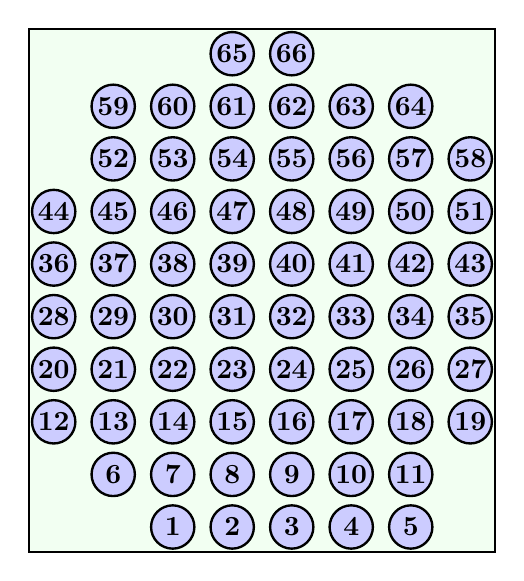
\begin{tikzpicture}[-,red, line width=0.06cm,font=\bfseries,draw=black] 
	\tikzstyle{every node}=[circle,ultra thick,draw=black,fill=white,text=black,minimum size=0.55cm,line width=0.03cm,inner sep=0.8pt]
	\tikzstyle{HC} =[fill=blue!20] % HC = healthy control node
	\tikzstyle{DS} =[fill=blue!20]  % DS = disease node
	\matrix [rectangle,row sep=2.5pt, column sep=5pt,draw=black,fill=green!5,line width=0.025cm] % 
	{
				    ;&				;&				 ;& \node(65)[HC]{65} ;& \node(66)[HC]{66} ;\\
		 		    ;& \node(59)[HC]{59} ;& \node(60)[HC]{60} ;& \node(61)[HC]{61} ;& \node(62)[HC]{62} ;& \node(63)[HC]{63} ;& \node(64)[HC]{64} ;& ;\\
		 		    ;& \node(52)[HC]{52} ;& \node(53)[HC]{53} ;& \node(54)[HC]{54} ;& \node(55)[HC]{55} ;& \node(56)[DS]{56} ;& \node(57)[HC]{57} ;& \node(58)[HC]{58} ;\\
	 \node(44)[HC]{44} ;& \node(45)[HC]{45} ;& \node(46)[HC]{46} ;& \node(47)[HC]{47} ;& \node(48)[DS]{48} ;& \node(49)[DS]{49} ;& \node(50)[DS]{50} ;& \node(51)[HC]{51} ;\\
	 \node(36)[HC]{36} ;& \node(37)[HC]{37} ;& \node(38)[HC]{38} ;& \node(39)[HC]{39} ;& \node(40)[HC]{40} ;& \node(41)[DS]{41} ;& \node(42)[HC]{42} ;& \node(43)[HC]{43} ;\\
	 \node(28)[HC]{28} ;& \node(29)[HC]{29} ;& \node(30)[HC]{30} ;& \node(31)[HC]{31} ;& \node(32)[HC]{32} ;& \node(33)[HC]{33} ;& \node(34)[HC]{34} ;& \node(35)[HC]{35} ;\\
	 \node(20)[HC]{20} ;& \node(21)[HC]{21} ;& \node(22)[HC]{22} ;& \node(23)[DS]{23} ;& \node(24)[HC]{24} ;& \node(25)[HC]{25} ;& \node(26)[HC]{26} ;& \node(27)[HC]{27} ;\\
	 \node(12)[HC]{12} ;& \node(13)[HC]{13} ;& \node(14)[DS]{14} ;& \node(15)[DS]{15} ;& \node(16)[DS]{16} ;& \node(17)[HC]{17} ;& \node(18)[HC]{18} ;& \node(19)[HC]{19} ;\\
		 		    ;& \node(6)[HC]{6} 	;& \node(7)[HC]{7} 	 ;& \node(8)[DS]{8}	  ;& \node(9)[HC]{9}   ;& \node(10)[HC]{10} ;& \node(11)[HC]{11} ;&  ;\\
	 			    ;&				;& \node(1)[HC]{1} 	 ;& \node(2)[HC]{2}	  ;& \node(3)[HC]{3}   ;& \node(4)[HC]{4}   ;& \node(1)[HC]{5}   ;&  ;\\
	};
\end{tikzpicture}
}
		 \caption{Control}
		 \label{subfig:sim,conn,struct,hc}
	\end{subfigure}
	\hspace{-4pt}
	\begin{subfigure}[b]{0.5\linewidth}
		 \centering
		 \resizebox{0.94\linewidth}{!}{%!TEX root = paper.tex
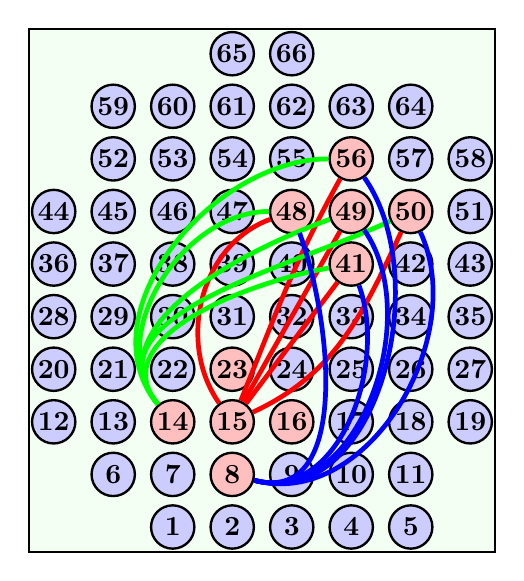
\begin{tikzpicture}[-,red, line width=0.06cm,font=\bfseries,draw=black] 
	\tikzstyle{every node}=[circle,ultra thick,draw=black,fill=white,text=black,minimum size=0.55cm,line width=0.03cm,inner sep=0.8pt]
	\tikzstyle{HC} =[fill=blue!20] % HC = healthy control node
	\tikzstyle{DS} =[fill=red!25]  % DS = disease node
	\matrix [rectangle,row sep=2.5pt, column sep=5pt,draw=black,fill=green!5,line width=0.025cm] % 
	{
				    ;&				;&				 ;& \node(65)[HC]{65} ;& \node(66)[HC]{66} ;\\
		 		    ;& \node(59)[HC]{59} ;& \node(60)[HC]{60} ;& \node(61)[HC]{61} ;& \node(62)[HC]{62} ;& \node(63)[HC]{63} ;& \node(64)[HC]{64} ;& ;\\
		 		    ;& \node(52)[HC]{52} ;& \node(53)[HC]{53} ;& \node(54)[HC]{54} ;& \node(55)[HC]{55} ;& \node(56)[DS]{56} ;& \node(57)[HC]{57} ;& \node(58)[HC]{58} ;\\
	 \node(44)[HC]{44} ;& \node(45)[HC]{45} ;& \node(46)[HC]{46} ;& \node(47)[HC]{47} ;& \node(48)[DS]{48} ;& \node(49)[DS]{49} ;& \node(50)[DS]{50} ;& \node(51)[HC]{51} ;\\
	 \node(36)[HC]{36} ;& \node(37)[HC]{37} ;& \node(38)[HC]{38} ;& \node(39)[HC]{39} ;& \node(40)[HC]{40} ;& \node(41)[DS]{41} ;& \node(42)[HC]{42} ;& \node(43)[HC]{43} ;\\
	 \node(28)[HC]{28} ;& \node(29)[HC]{29} ;& \node(30)[HC]{30} ;& \node(31)[HC]{31} ;& \node(32)[HC]{32} ;& \node(33)[HC]{33} ;& \node(34)[HC]{34} ;& \node(35)[HC]{35} ;\\
	 \node(20)[HC]{20} ;& \node(21)[HC]{21} ;& \node(22)[HC]{22} ;& \node(23)[DS]{23} ;& \node(24)[HC]{24} ;& \node(25)[HC]{25} ;& \node(26)[HC]{26} ;& \node(27)[HC]{27} ;\\
	 \node(12)[HC]{12} ;& \node(13)[HC]{13} ;& \node(14)[DS]{14} ;& \node(15)[DS]{15} ;& \node(16)[DS]{16} ;& \node(17)[HC]{17} ;& \node(18)[HC]{18} ;& \node(19)[HC]{19} ;\\
		 		    ;& \node(6)[HC]{6} 	;& \node(7)[HC]{7} 	 ;& \node(8)[DS]{8}	  ;& \node(9)[HC]{9}   ;& \node(10)[HC]{10} ;& \node(11)[HC]{11} ;&  ;\\
	 			    ;&				;& \node(1)[HC]{1} 	 ;& \node(2)[HC]{2}	  ;& \node(3)[HC]{3}   ;& \node(4)[HC]{4}   ;& \node(1)[HC]{5}   ;&  ;\\
	};
	% edge group red
	\tikzstyle{col}=[red] 
	\draw(15)to[](41)[col];
	\draw(15)to[out=125,in=-160](48)[col];
	\draw(15)to[](49)[col];
	\draw(15)to[out=25,in=-115](50)[col];
	\draw(15)to[out=68,in=-119](56)[col];
	% edge group green
	\tikzstyle{col}=[green!100] 
	\draw(14)to[out=130,in=190](41)[col];
	\draw(14)to[out=130,in=180](48)[col];
	\draw(14)to[out=130,in=200](49)[col];
	\draw(14)to[out=130,in=205](50)[col];
	\draw(14)to[out=130,in=180](56)[col];	
	% edge group blue
	\tikzstyle{col}=[blue] 
	\draw(8)to[out=-15,in=-70](41)[col];
	\draw(8)to[out=-15,in=-70](48)[col];
	\draw(8)to[out=-15,in=-55](49)[col];
	\draw(8)to[out=-15,in=-65](50)[col];
	\draw(8)to[out=-15,in=-55](56)[col];
\end{tikzpicture}
\begin{tikzpicture}[-,red, line width=0.06cm,font=\bfseries,draw=black] 
	\tikzstyle{every node}=[circle,ultra thick,draw=black,fill=white,text=black,minimum size=0.55cm,line width=0.03cm,inner sep=0.8pt]
	\tikzstyle{HC} =[fill=blue!20] % HC = healthy control node
	\tikzstyle{DS} =[fill=red!25]  % DS = disease node
	\matrix [rectangle,row sep=2.5pt, column sep=5pt,draw=black,fill=green!5,line width=0.025cm] % 
	{
				    ;&				;&				 ;& \node(65)[HC]{65} ;& \node(66)[HC]{66} ;\\
		 		    ;& \node(59)[HC]{59} ;& \node(60)[HC]{60} ;& \node(61)[HC]{61} ;& \node(62)[HC]{62} ;& \node(63)[HC]{63} ;& \node(64)[HC]{64} ;& ;\\
		 		    ;& \node(52)[HC]{52} ;& \node(53)[HC]{53} ;& \node(54)[HC]{54} ;& \node(55)[HC]{55} ;& \node(56)[DS]{56} ;& \node(57)[HC]{57} ;& \node(58)[HC]{58} ;\\
	 \node(44)[HC]{44} ;& \node(45)[HC]{45} ;& \node(46)[HC]{46} ;& \node(47)[HC]{47} ;& \node(48)[DS]{48} ;& \node(49)[DS]{49} ;& \node(50)[DS]{50} ;& \node(51)[HC]{51} ;\\
	 \node(36)[HC]{36} ;& \node(37)[HC]{37} ;& \node(38)[HC]{38} ;& \node(39)[HC]{39} ;& \node(40)[HC]{40} ;& \node(41)[DS]{41} ;& \node(42)[HC]{42} ;& \node(43)[HC]{43} ;\\
	 \node(28)[HC]{28} ;& \node(29)[HC]{29} ;& \node(30)[HC]{30} ;& \node(31)[HC]{31} ;& \node(32)[HC]{32} ;& \node(33)[HC]{33} ;& \node(34)[HC]{34} ;& \node(35)[HC]{35} ;\\
	 \node(20)[HC]{20} ;& \node(21)[HC]{21} ;& \node(22)[HC]{22} ;& \node(23)[DS]{23} ;& \node(24)[HC]{24} ;& \node(25)[HC]{25} ;& \node(26)[HC]{26} ;& \node(27)[HC]{27} ;\\
	 \node(12)[HC]{12} ;& \node(13)[HC]{13} ;& \node(14)[DS]{14} ;& \node(15)[DS]{15} ;& \node(16)[DS]{16} ;& \node(17)[HC]{17} ;& \node(18)[HC]{18} ;& \node(19)[HC]{19} ;\\
		 		    ;& \node(6)[HC]{6} 	;& \node(7)[HC]{7} 	 ;& \node(8)[DS]{8}	  ;& \node(9)[HC]{9}   ;& \node(10)[HC]{10} ;& \node(11)[HC]{11} ;&  ;\\
	 			    ;&				;& \node(1)[HC]{1} 	 ;& \node(2)[HC]{2}	  ;& \node(3)[HC]{3}   ;& \node(4)[HC]{4}   ;& \node(1)[HC]{5}   ;&  ;\\
	};
	%********************** Style 2 **************************%
%	% edge group red
	\tikzstyle{col}=[black] 
	\draw(23)to[out=15,in=-90](41)[col];
	\draw(23)to[](48)[col];
	\draw(23)to[](49)[col];
	\draw(23)to[out=0,in=-90](50)[col];
	\draw(23)to[out=90,in=180](56)[col];

	% edge group yellow
	\tikzstyle{col}=[myorange] 
	\draw(16)to[in=-80](41)[col];
	\draw(16)to[](48)[col];
	\draw(16)to[out=78,in=-120](49)[col];
	\draw(16)to[out=30,in=-80](50)[col];
	\draw(16)to[out=82,in=-123](56)[col];
\end{tikzpicture}
}
		 \caption{Patient}
		 \label{subfig:sim,conn,struct,ds}
	\end{subfigure}
	\begin{subfigure}[b]{0.235\linewidth}
		 \centering
		 \raisebox{0pt}{\hspace{-8pt}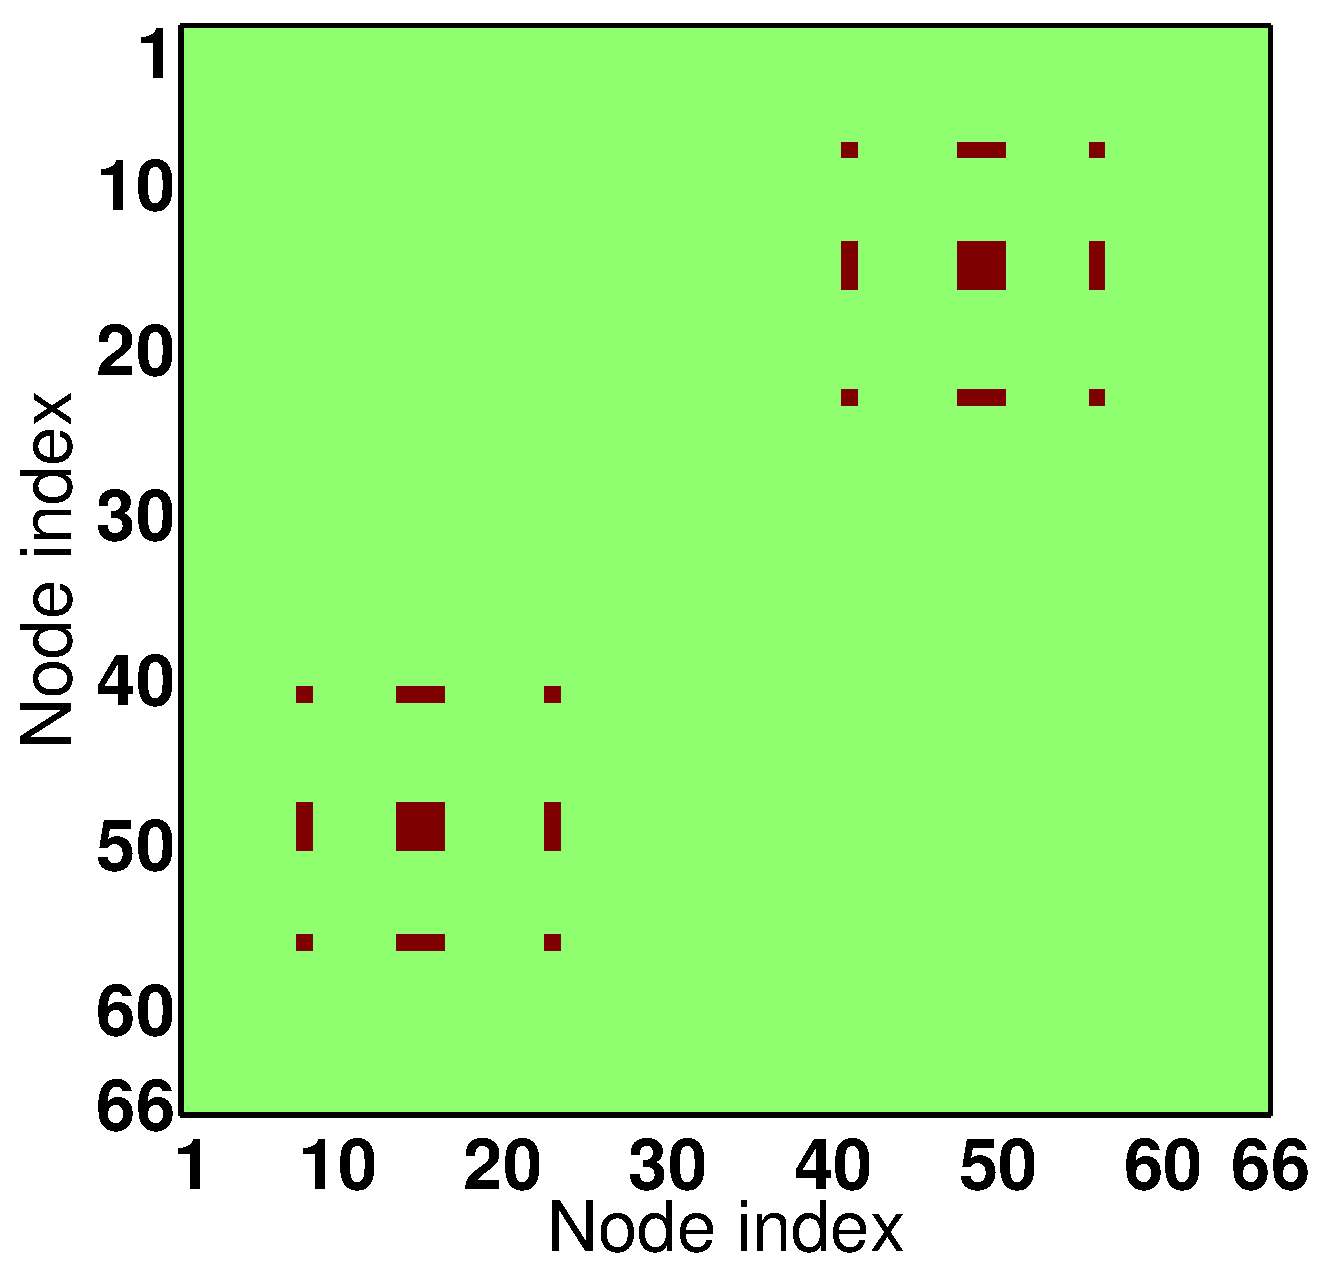
\includegraphics[width=1.125\linewidth]{\fig/sim_weight_truth.pdf}}\vspace{-5pt}\\
		 \caption{Edge support}
		 \label{subfig:sim,conn,struct,supp}
	\end{subfigure}
	\vspace{-12pt}
	\caption{
		Schematic representations of the synthetic $4$-D functional connectome data generated for the simulation experiments (best viewed in color). 
		(a) Node orientation representing the ``control class'' connectome, where the blue nodes indicate
the normal nodes.
		(b) Node orientation representing the ``patient class'' connectome, where there are $25$ \emph{anomalous edges} shared among the two \emph{anomalous node} clusters indicated in red (this subfigure is split into two side-by-side figures to improve visibility of the impacted edges).
		(c) Binary support matrix indicating the locations of the anomalous edges in the connectome space.
	}
	\label{fig:sim,conn,struct}
\end{figure}
%****************************************************************%

It is important to note that the inclusion of the clusters of anomalous nodes is motivated from the ``patchiness assumption'' of brain disorders, a view that has been born from multiple task-based and connectivity-based studies; this point will be expounded in finer detail in \ref{subsec:why,flasso}.
In short, the ``patchiness assumption'' is the view that major psychiatric disorders manifest in the brain by impacting moderately sized spatially contiguous regions,  which is what the clusters of anomalous nodes are intended to mimic in this simulation.

For training the classifiers, we sampled $100$ functional connectomes consisting of $50$ control samples and $50$ patient samples. 
For evaluating the performance of the classifiers, we sampled $500$ additional functional connectomes consisting of $250$ control samples and $250$ patient samples.


%===================================================================%
% Real-data  experiment setup
%===================================================================%
\subsection{Real experimental data: schizophrenia resting state dataset}
\label{subsec:real,data}
%!TEX root = paper.tex
%===================================================================%
% Real data info
%===================================================================%
To further assess the utility of the proposed method, we also conducted experiments on real resting state scans.

\paragraph{Participants}
We used the Center for Biomedical Research Excellence (COBRE) dataset (\url{http://fcon_1000.projects.nitrc.org/indi/retro/cobre.html}) made available by the Mind Research Network. 
The dataset is comprised of $74$ typically developing control participants and $71$ participants with a DSM-IV-TR diagnosis of schizophrenia. 
Diagnosis was established by the Structured Clinical Interview for DSM-IV (SCID). Participants were excluded if they had mental retardation, neurological disorder, head trauma, or substance abuse or dependence in the last $12$ months. A summary of the participant demographic characteristics is provided in Table~\ref{table:schiz,demographic}. 

\paragraph{Data Acquisition}
A multi-echo MPRAGE (MEMPR) sequence was used with the following parameters: TR/TE/TI = $2530/[1.64, 3.5, 5.36, 7.22, 9.08]$/$900$ ms, flip angle $= 7^{\circ}$, FOV $= 256\times 256$ mm, slab thickness $= 176$ mm, matrix size $= 256\times 256\times 176$, voxel size $= 1\times 1\times 1$ mm, number of echoes $= 5$, pixel bandwidth $=650$ Hz, total scan time $= 6$ minutes. 
With $5$ echoes, the TR and TI time to encode partitions for the MEMPR are similar to that of a conventional MPRAGE, resulting in similar GM/WM/CSF contrast. 
Resting state data were collected with single-shot full k-space echo-planar imaging (EPI) with ramp sampling correction using the intercomissural line (AC-PC) as a reference (TR: $2$ s, TE: $29$ ms, matrix size: $64\times 64$, $32$ slices, voxel size: $3\times 3\times 4 mm^3$).

\paragraph{Imaging Sample Selection}
Analyses were limited to participants with: 
(1) MPRAGE anatomical images, with consistent near-full brain coverage (\ie, superior extent included the majority of frontal and parietal cortex and inferior extent included the temporal lobes) with successful registration; 
(2) complete phenotypic information for main phenotypic variables (diagnosis, age, handedness); 
(3) mean framewise displacement (FD) within two standard deviations of the sample mean; 
(4) at least $50\%$ of frames retained after application of framewise censoring for motion (``motion scrubbing''; see below).
After applying these sample selection criteria, we analyzed resting state scans from $121$ individuals consisting of $67$ healthy controls (HC) and $54$ schizophrenic subjects (SZ). 
Demographic characteristics of the post-exclusion sample are shown in Table~\ref{table:schiz,demographic}.

%=================================================================== 
\newcommand{\mycellcol}{\cellcolor{blue!25}}
\begin{table}[t!]
	\centering
	\begin{tabular}{l|cccc|cccc}
		\multicolumn{1}{c}{}&\multicolumn{4}{c}{\textbf{Healthy Controls}}&\multicolumn{4}{c}{\textbf{Schizophrenia}}\\
		\hline
			& $n$ & Age & \#male & \#RH & $n$ & Age & \#male & \#RH \\		
		\hline\hline
		 Pre-exclusion 	& $74$ & $35.8\pm 11.6$ & $51$ & $71$ 
		 		  		& $71$ & $38.1\pm 14.0$ & $57$ & $59$ \\
		 Post-exclusion 	& $67$ & $35.2\pm 11.7$ & $46$ & $66$ 
		 				& $54$ & $35.5\pm 13.1$ & $48$ & $46$ \\
		\hline
	\end{tabular}
	\caption{
		Demographic characteristics of the participants before and after sample exclusion criteria is applied \mbox{(RH = right-handed)}.
	}
	\label{table:schiz,demographic}
\end{table}
%=================================================================== 

\paragraph{Preprocessing}
Preprocessing steps were performed using statistical parametric mapping (SPM$8$; \url{www.fil.ion.ucl.ac.uk/spm}). 
Scans were reconstructed, slice-time corrected, realigned to the first scan in the experiment for correction of head motion, and co-registered with the high-resolution T$1$-weighted image. 
Normalization was performed using the voxel-based morphometry (VBM) toolbox implemented in SPM$8$. 
The high-resolution T$1$-weighted image was segmented into tissue types, bias-corrected, registered to MNI space, and then normalized using Diffeomorphic Anatomical Registration Through Exponentiated Lie Algebra (DARTEL) \citep{Ashburner:2007}. 
The resulting deformation fields were then applied to the functional images. 
Smoothing of functional data was performed with an $8$ mm$^3$ kernel.

\paragraph{Connectome generation}
Functional connectomes were generated by placing $7.5$ mm radius nodes representing ROIs encompassing $33$ $3\times 3\times 3$ mm voxels in a regular grid spaced at $18\times 18 \times 18$~mm intervals throughout the brain. 
Spatially averaged time series were extracted from each of the ROIs. 
Next, linear detrending was performed, followed by nuisance regression. 
Regressors included six motion regressors generated from the realignment step, as well as their first derivatives. 
White matter and cerebrospinal fluid masks were generated from the VBM-based tissue segmentation step noted above, and eroded using the \textsf{fslmaths} program from FSL to eliminate border regions of potentially ambiguous tissue type. 
The top five principal components of the BOLD time series were extracted from each of the masks and included as regressors in the model -- a method that has been demonstrated to effectively remove signals arising from the cardiac and respiratory cycle \citep{Behzadi:2007}. 
The time-series for each ROI was then band-passed filtered in the $0.01$ -- $0.10$ Hz range. 
Individual frames with excessive head motion were then censored from the time series. 
Subjects with more than $50\%$ of their frames removed by scrubbing were excluded from further analysis, a threshold justified by simulations conducted by other groups \citep{Fair:2013}, as well as by our group. 
Pearson product-moment correlation coefficients were then calculated pairwise between time courses for each of the $347$ ROIs.
Standard steps in functional connectivity analysis (removing motion artifacts and nuisance covariates and calculating Pearson's product moment correlations between pairs of nodes) was performed with \texttt{ConnTool}, a functional connectivity analysis package developed by Robert C. Welsh, University of Michigan.

